\newcommand{\msa}{\mathcal{M}_1}
\newcommand{\msb}{\mathcal{M}_2}
\newcommand{\eexp}{E_\text{exp}}
\newcommand{\evar}{E_\text{var}}

\section{Methods}
\label{s:method}
In this section, we first focus on the method of data assimilation based on Kalman filter. 
Since this area of research is vast, we present only 
brief description of the related methods and refer the reader to a detailed introduction to
filtering methods available for example in~\cite{grewal2014kalman, welch2006introduction}. Then, we focus on the 
recently developed \emph{reduced-order} varian of the unscented Kalman filter which is in the core of our work. 
Finally, we describe the model of deformable objects 
based on the finite-element formulation of the elasticity problem. 

%%%%%%%%%%%%%%%%%%%%%%%%%%% KF:

\subsection{Data Assimilation Based on Kalman Filtering}
\label{sm:kalman}
One of the important data assimilation techniques is \emph{Kalman filtering},
%\footnote{The word \emph{filter} comes from the Kalman Filter's ability to filter out measurement noise, thus smoothing the simulation.} 
an algorithm first proposed by R. E. K\'{a}lm\'{a}n in 1960~\cite{kalman1960new}. The algorithm specifies a set of equations to be used for the prediction and correction steps. The reasoning behind the equations is based on a number of assumptions, under which the filter is in fact an optimal algorithm. Namely, these assumptions include  that the measurements are linked to the state of the model with linear equations, and that the state evolution of the model is also governed by linear equations.

The usefulness of Kalman filter was quickly recognized: the algorithm is especially suitable for real-time applications thanks to its low computational complexity as well as recursive nature. These features, highly desirable in many other applications, have encouraged the use of Kalman filter even for non-linear systems. To improve the algorithm's performance on these systems, a modification now known as \emph{extended Kalman filter} (EKF) was designed already in the 1960s. The EKF is based on the idea of linearizing the estimation around the current estimate in something akin to Taylor series \cite{welch2006introduction}. Notably, this modification retains the low computational demands of the original Kalman filter, although it requires mode intensive computations performed by the model which has to provide the Jacobian of the model function. 

The EKF and its numerous modifications have since claimed a central role in several applications such as the navigation systems and GPS. However, much like any approach based on Taylor series, this approach is particularly suitable when the time step is small enough; if only the first derivation is used, the function has to be \emph{almost linear} in the interval. If the non-linearity of the function dominates our computational capabilities (the step cannot be made small enough), the EKF is known to propagate the probability distributions of variables inaccurately, producing highly inaccurate results or even diverging~\cite{wan2000}.


%%%%%%%%%%%%%%%%%%%%%%%%%%% UKF:

\subsection{Unscented Kalman Filter}
\label{sm:UKF}
Whereas EKF is a rather straightforward application of basics of basic calculus and appeared shortly after the KF was designed, the \emph{Unscented Kalman Filter} (UKF) was designed by Julier and Uhlmann only in 1997 \cite{julier1997new}. The UKF is based on the idea that it is easier to approximate a probability distribution than it is to approximate a function.  The state estimate distribution is again approximated by a Gaussian random variable
%\footnote{A Gaussian random variable is nickname for a random variable with normal probability distribution.}
(GRV), but this GRV is represented by a set of sample points, called \emph{sigma points}. The sigma points, when propagated through the \emph{genuine} non-linear system, achieve third-order accuracy \cite{wan2000} for \emph{any} nonlinear system. Remarkably, the computational complexity of UKF is asymptotically equal to that of EKF. Detailed derivations of the filter and comparison to other methods can be found in~\cite{julier2004unscented,wan2000}.

The scenario considered here is governed by \emph{non-linear} stochastic equation:
\begin{equation*}
\mathbf{x}_{n+1} = f(\mathbf{x}_{n}) + \mathbf{w}_{n}\,,
\end{equation*}
where $\mathbf{x}_n \in \mathbb{R}^p$ is the state of the assimilated model. The measurement is given by
\begin{equation*}
\mathbf{z}_n = h(\mathbf{x}_{n}) + \mathbf{v}_{n}\,.
\end{equation*}
where $\mathbf{z}_n$ is usually referenced as the \emph{innovation} necessary for computation of the correction via Kalman gain.
Both the errors are again Gaussian with zero mean and with co-variance matrices $\mathbf{Q}$ and $\mathbf{R}$ respectively. 

The UKF makes use of \emph{sigma points}, and thereby evaluates the model using a number "nearby" states and inferring its view of the situation from all these results along with the observations. To specify the UKF, we thus first explain what sigma points are and how they are obtained. Thereafter the modified prediction and correction step equations are presented. 

%\subsubsection{Sigma points}
Consider a random variable $\mathbf{x} \in \mathbb{R}^p$ and the derived random variable $\mathbf{x}_f = f(\mathbf{x})$, where $f$ is nonlinear. Sigma points $\mathbf{x}^{[i]}$ together with their weights essentially represent a probability distribution on a finite number of "noised" state vectors. The distribution satisfies a number of assumptions, which ensure that (1) the distribution has the same mean and co-variance matrix as $\mathbf{x}$, and (2) the distribution accurately approximates that of the transformed variable $\mathbf{x_f}$. The accuracy is to the second order for arbitrary $\mathbf{x}$ , and to third order if $\mathbf{x}$ is Gaussian~\cite{wan2000}.

We refer to a set of $r$ points $\mathbf{x}^{[i]}$ with weights $\alpha_i$, where the points can be expressed by
\begin{equation*}
\mathbf{x}^{[i]} = \ev (X) + \tilde{\mathbf{x}}^{[i]} \,,
\quad
1 \leq i \leq r \,,
\end{equation*}
as \emph{sigma points} if the following criteria are simultaneously met:
\begin{flalign}
\label{SP1}
\sum\limits_{i=1}^{r} \alpha_i &=1 \,\\
\label{SP2}
\ev_\alpha (\mathbf{X^*}) \defeq \sum\limits_{i=1}^{r} \alpha_i \mathbf{x}^{[i]} &= \ev(\mathbf{x})\,\\
\label{SP3}
\Cov_\alpha (\mathbf{X^*})  \defeq \sum\limits_{i=1}^{r} \alpha_i (\mathbf{x}^{[i]}- \ev (\mathbf{x})) \cdot (\mathbf{x}^{[i]}- \ev (\mathbf{x})) ^{\sf T} &= \Cov (\mathbf{x})
\end{flalign}
Here, $\mathbf{X}^* = \begin{bmatrix} \mathbf{x}^{[0]} ... \mathbf{x}^{[r-1]} \end{bmatrix}$ denotes the \emph{sigma point matrix}.
Note that the sigma points themselves are \emph{not} random variables. Assuming Equations \ref{SP1}, \ref{SP2} and \ref{SP3} hold, the following expressions trivially hold:
\begin{flalign*}
\sum\limits_{i=1}^{r} \alpha_i \mathbf{\tilde{x}}^{[i]} &= \mathbf{0}\,\\
\sum\limits_{i=1}^{r} \alpha_i \mathbf{\tilde{x}}^{[i]} \cdot ( {\mathbf{\tilde{x}}^{[i]}} )^{\sf T} &= \Cov(\mathbf{x}) \,.
\end{flalign*}
It can also be shown that
\begin{flalign*}
\ev_\alpha  (\mathbf{X^*}) &= \ev (\mathbf{x}_f) + o\left( \ev (\norm{\mathbf{\tilde{x}}}^2)\right) \,,\\
\Cov_\alpha   (\mathbf{X^*}) &= \Cov (\mathbf{x}_f) + o\left( \ev (\norm{\mathbf{\tilde{x}}}^2)\right) \,,
\end{flalign*}
which is exactly what we expect from the sigma points.

The system of Equations \ref{SP1}, \ref{SP2} and \ref{SP3} has an infinite number of solutions, especially as the number of sigma points may be arbitrary. We  present the three most popular heuristics, in terms of their position relative to the mean. These relative positions are represented as columns $\mathbf{I}^{[i]}$ of matrix $I$.
\begin{itemize}
\item \emph{simplex sigma points}: This heuristic determines $r=p+1$ sigma points where $p$ is the dimension of the state vector. Also note that $r=p+1$ is the smallest possible number of sigma points. The sigma points $\mathbf{I}^{[i]}$ form a regular polyhedron of radius $\sqrt{p}$ and $\alpha_i = \sfrac{1}{p}$.
\item \emph{canonical sigma points}: This heuristic determines $r=2p$ sigma points. The points are located at $\mathbf{I}^{[i]} = -\mathbf{I}^{[i+p]}= \sqrt{p} \cdot \mathbf{e}_i$, where $\{\mathbf{e}_i\}$ is an orthonormal basis of $\mathbb{R}^p$, and $\alpha_i = \sfrac{1}{2p}$.
\item \emph{star sigma points}: This heuristic determines $r=2p+1$ sigma points, located at $\mathbf{I}^{[i]} = -\mathbf{I}^{[i+p]}= \sqrt{p} \cdot \mathbf{e}_i$ and at $\mathbf{I}^{[2p+1]}=\mathbf{0}$. The value of $\alpha$ is $\alpha_i = \sfrac{1}{2p+1}$.
\end{itemize}
%These herustics for sigma points are illustrated in two dimensions in Figure \ref{sigsalabim}.
% \begin{figure}[ht]
%     \centering
%     \includegraphics[width=1.0\textwidth]{sigma.png}
%     \caption{Sigma point choices in two dimensions about the cross (mean). \textbf{blue:} simplex. \textbf{green:} canonical. \textbf{red:} star.}
% \label{sigsalabim}
% \end{figure}
Given the choice of sigma points, the unscented Kalman filter is given by following sets of equations, divided into the prediction and correction phase:

\subsubsection{UKF --- Prediction Step}

\begin{flalign}
\label{sampling}
\mathbf{\hat{x}}_n^{[i]+} &= \mathbf{\hat{x}}_n^{+} + \sqrt{\mathbf{P}_{n}^{+}}I^{[i]} \,,\\
\mathbf{\hat{x}}_{n+1}^{-} &= \ev_\alpha (f(\mathbf{\hat{x}}^{*+}_n))\,,\\
\mathbf{P}_{n+1}^{-} &= \Cov_\alpha(f(\mathbf{\hat{x}}_n^{*+})) + \mathbf{Q} \,,
\end{flalign}
The step described by Equation \ref{sampling} is sometimes referred to as \emph{sampling} -- its output are sigma points for the current step. Thereafter, the model is applied to
the sigma points, and the mean and covariance of the probability distribution on them is determined and saved as \emph{a priori} estimates.

\subsubsection{UKF --- Correction Step}
\begin{flalign}
\mathbf{\hat{x}}_{n+1}^{[i]-} &= \mathbf{\hat{x}}_{n+1}^{-}  + \sqrt{\mathbf{P}_{n+1}^{-}}I^{[i]} \,,\\
\mathbf{{z}}_{n+1}^{[i]} &= h (\mathbf{\hat{x}}_{n+1}^{[i]-})  \,,\\
\mathbf{P}_{\alpha}^{\tilde{x} \tilde{z}} &= \Cov_\alpha (\mathbf{z}_{n+1}^*, \mathbf{z}_{n+1}^*) \,,\\
\mathbf{P}_{\alpha}^{\tilde{z}} &= \mathbf{R}_{n+1} + \Cov_\alpha (\mathbf{z}_{n+1}^*, \mathbf{z}_{n+1}^*)\,,\\
 \mathbf{\hat{K}}_{n+1} &=  \mathbf{P}_{\alpha}^{\tilde{x} \tilde{z}} \cdot (\mathbf{P}_{\alpha}^{\tilde{z}} )^{-1} \,,\\
\label{UKFup1}
 \mathbf{\hat{x}}_{n+1}^+ &=  \mathbf{x}_{n}^{-} +  \mathbf{\hat{K}}_{n+1}  (\mathbf{z}_{n+1} - \ev_\alpha(\mathbf{z}^*_{n+1}))\,,\\
\label{UKFup2}
 \mathbf{\hat{P}}_{n+1}^+ &=  \mathbf{\hat{P}}_{n+1}^- -  \mathbf{P}_{\alpha}^{\tilde{x} \tilde{z}} \cdot
 (\mathbf{P}_{\alpha}^{\tilde{z}} )^{-1} (\mathbf{P}_{\alpha}^{\tilde{x} \tilde{z}})^{\sf T}\,.
\end{flalign}
Here, the Eq. 8 represents the computation of \emph{innovation} given by the function $h$ requiring the observations of the 
modeled phenomenon. 


\begin{figure*}[t!]%
\centering%
\subfigure[]{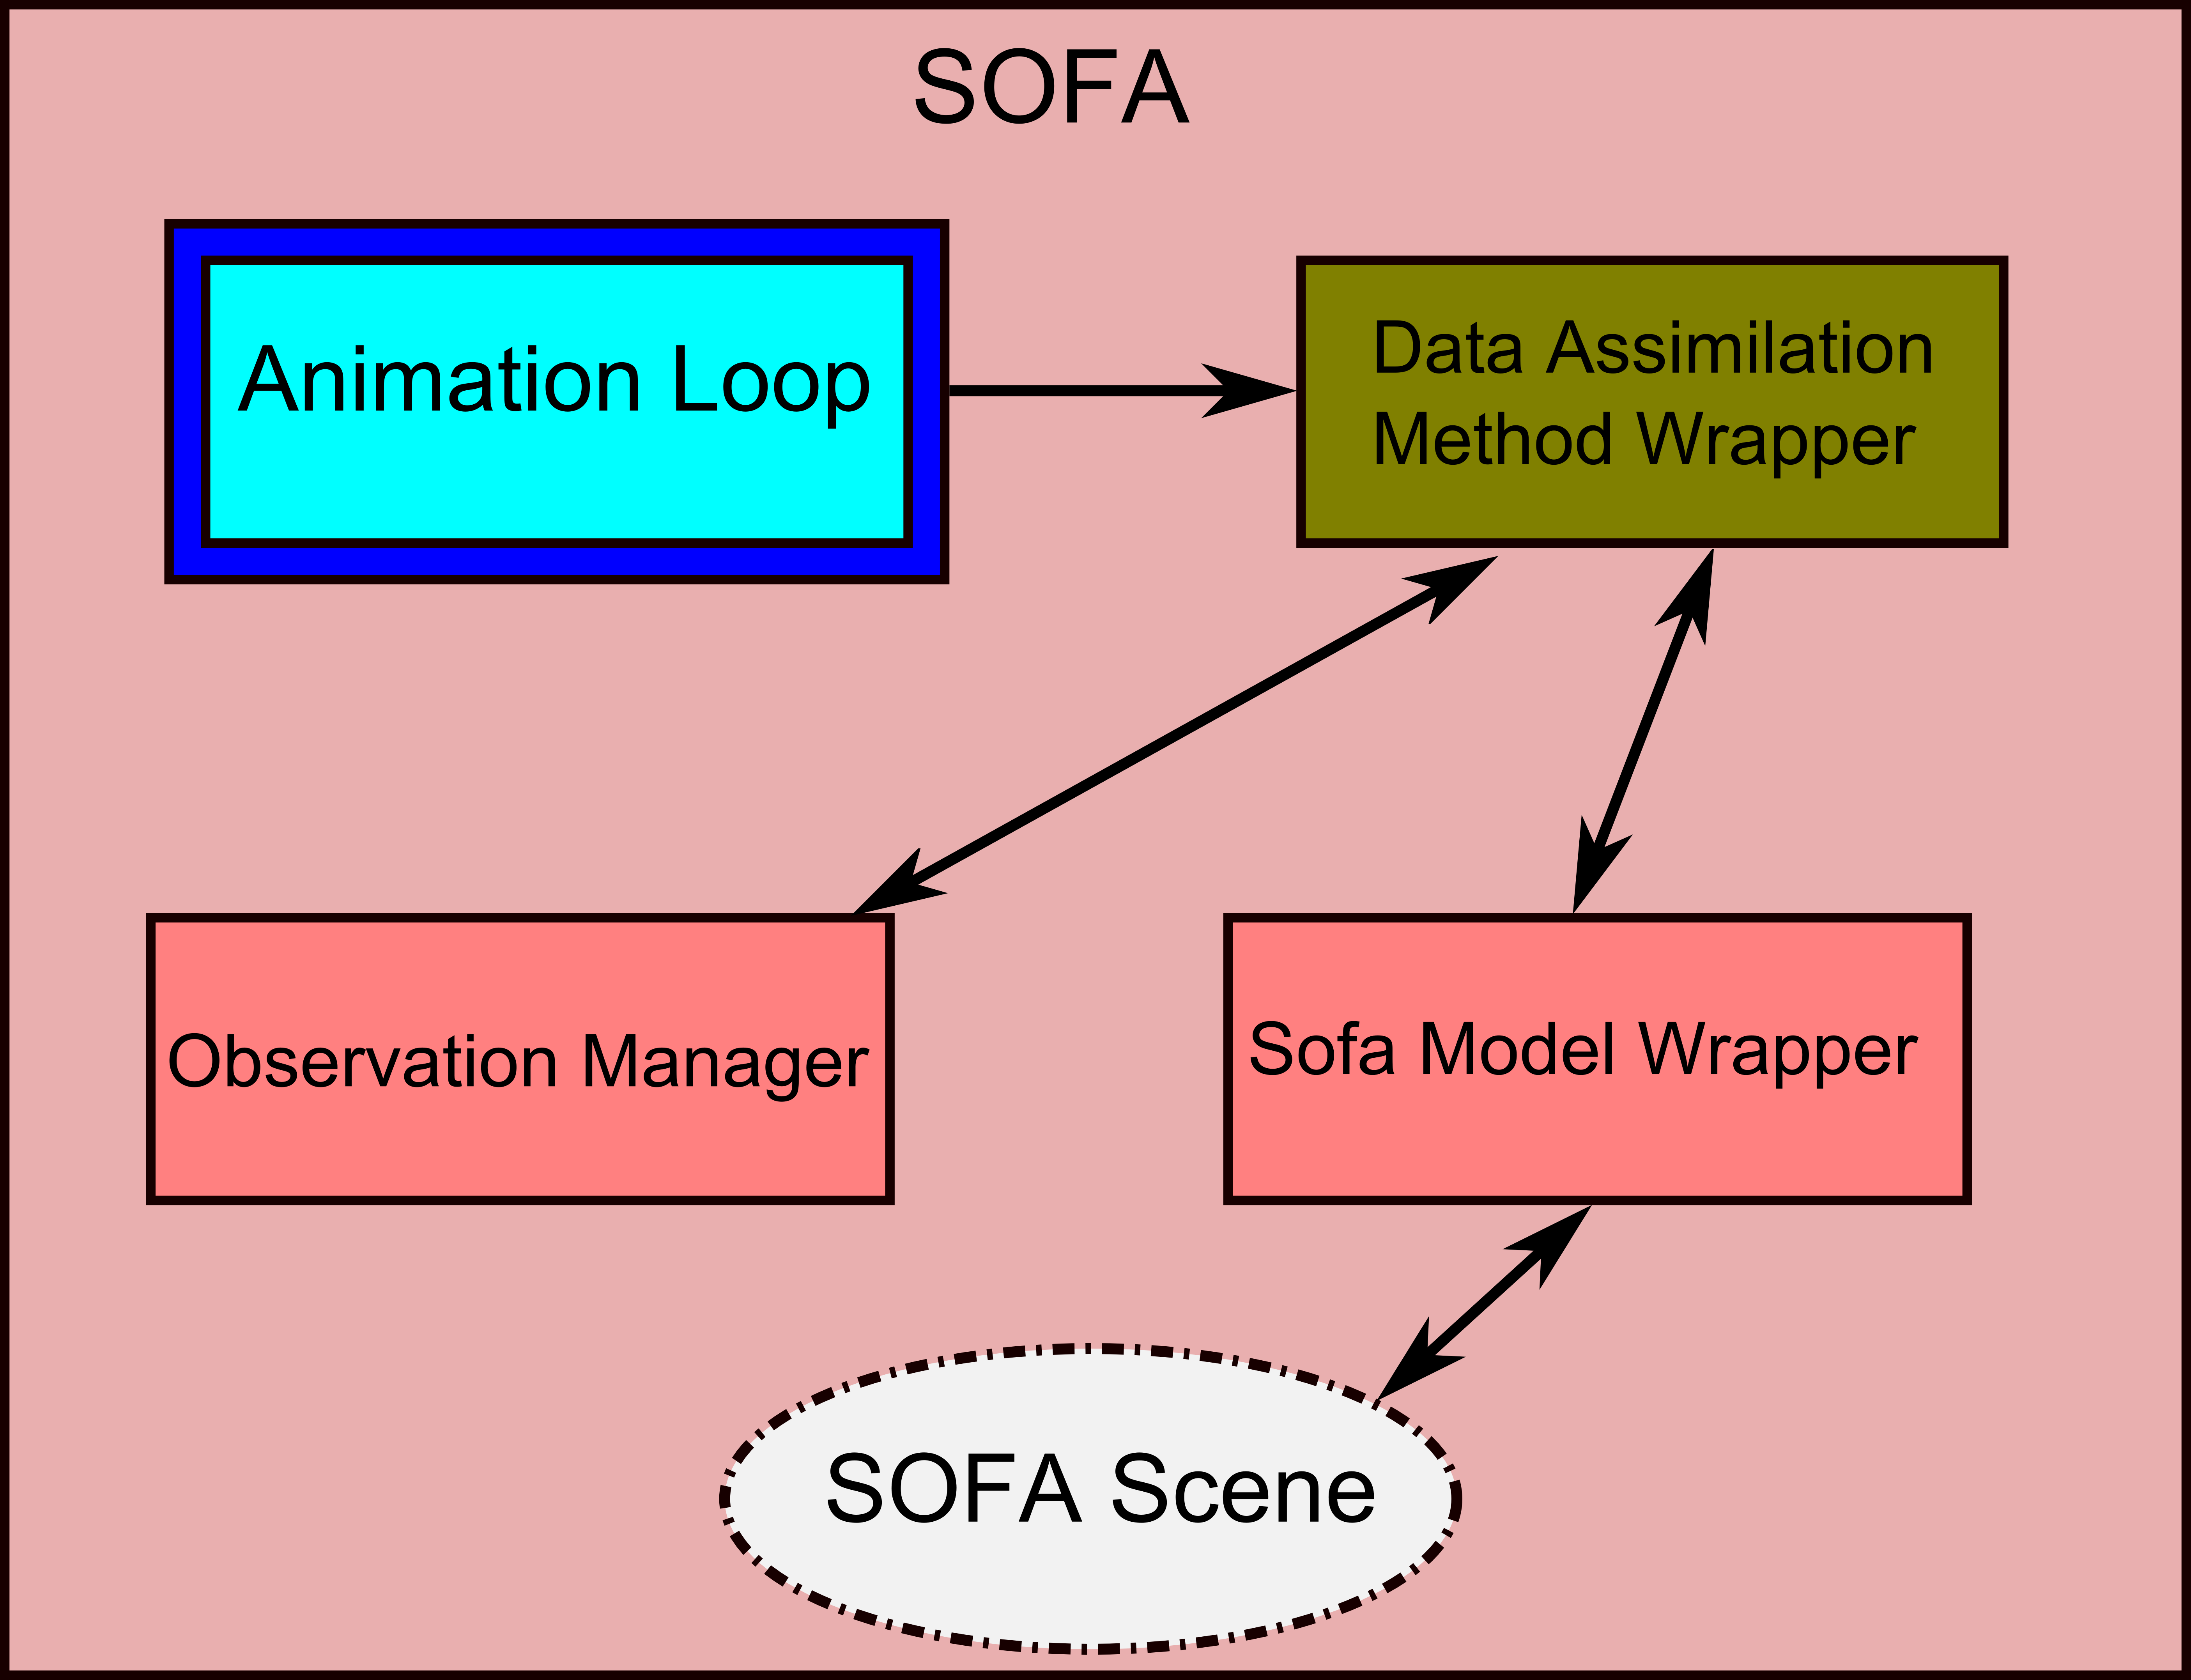
\includegraphics[height=4cm]{figs/integrationScheme1.png}}
\hfill
\subfigure[]{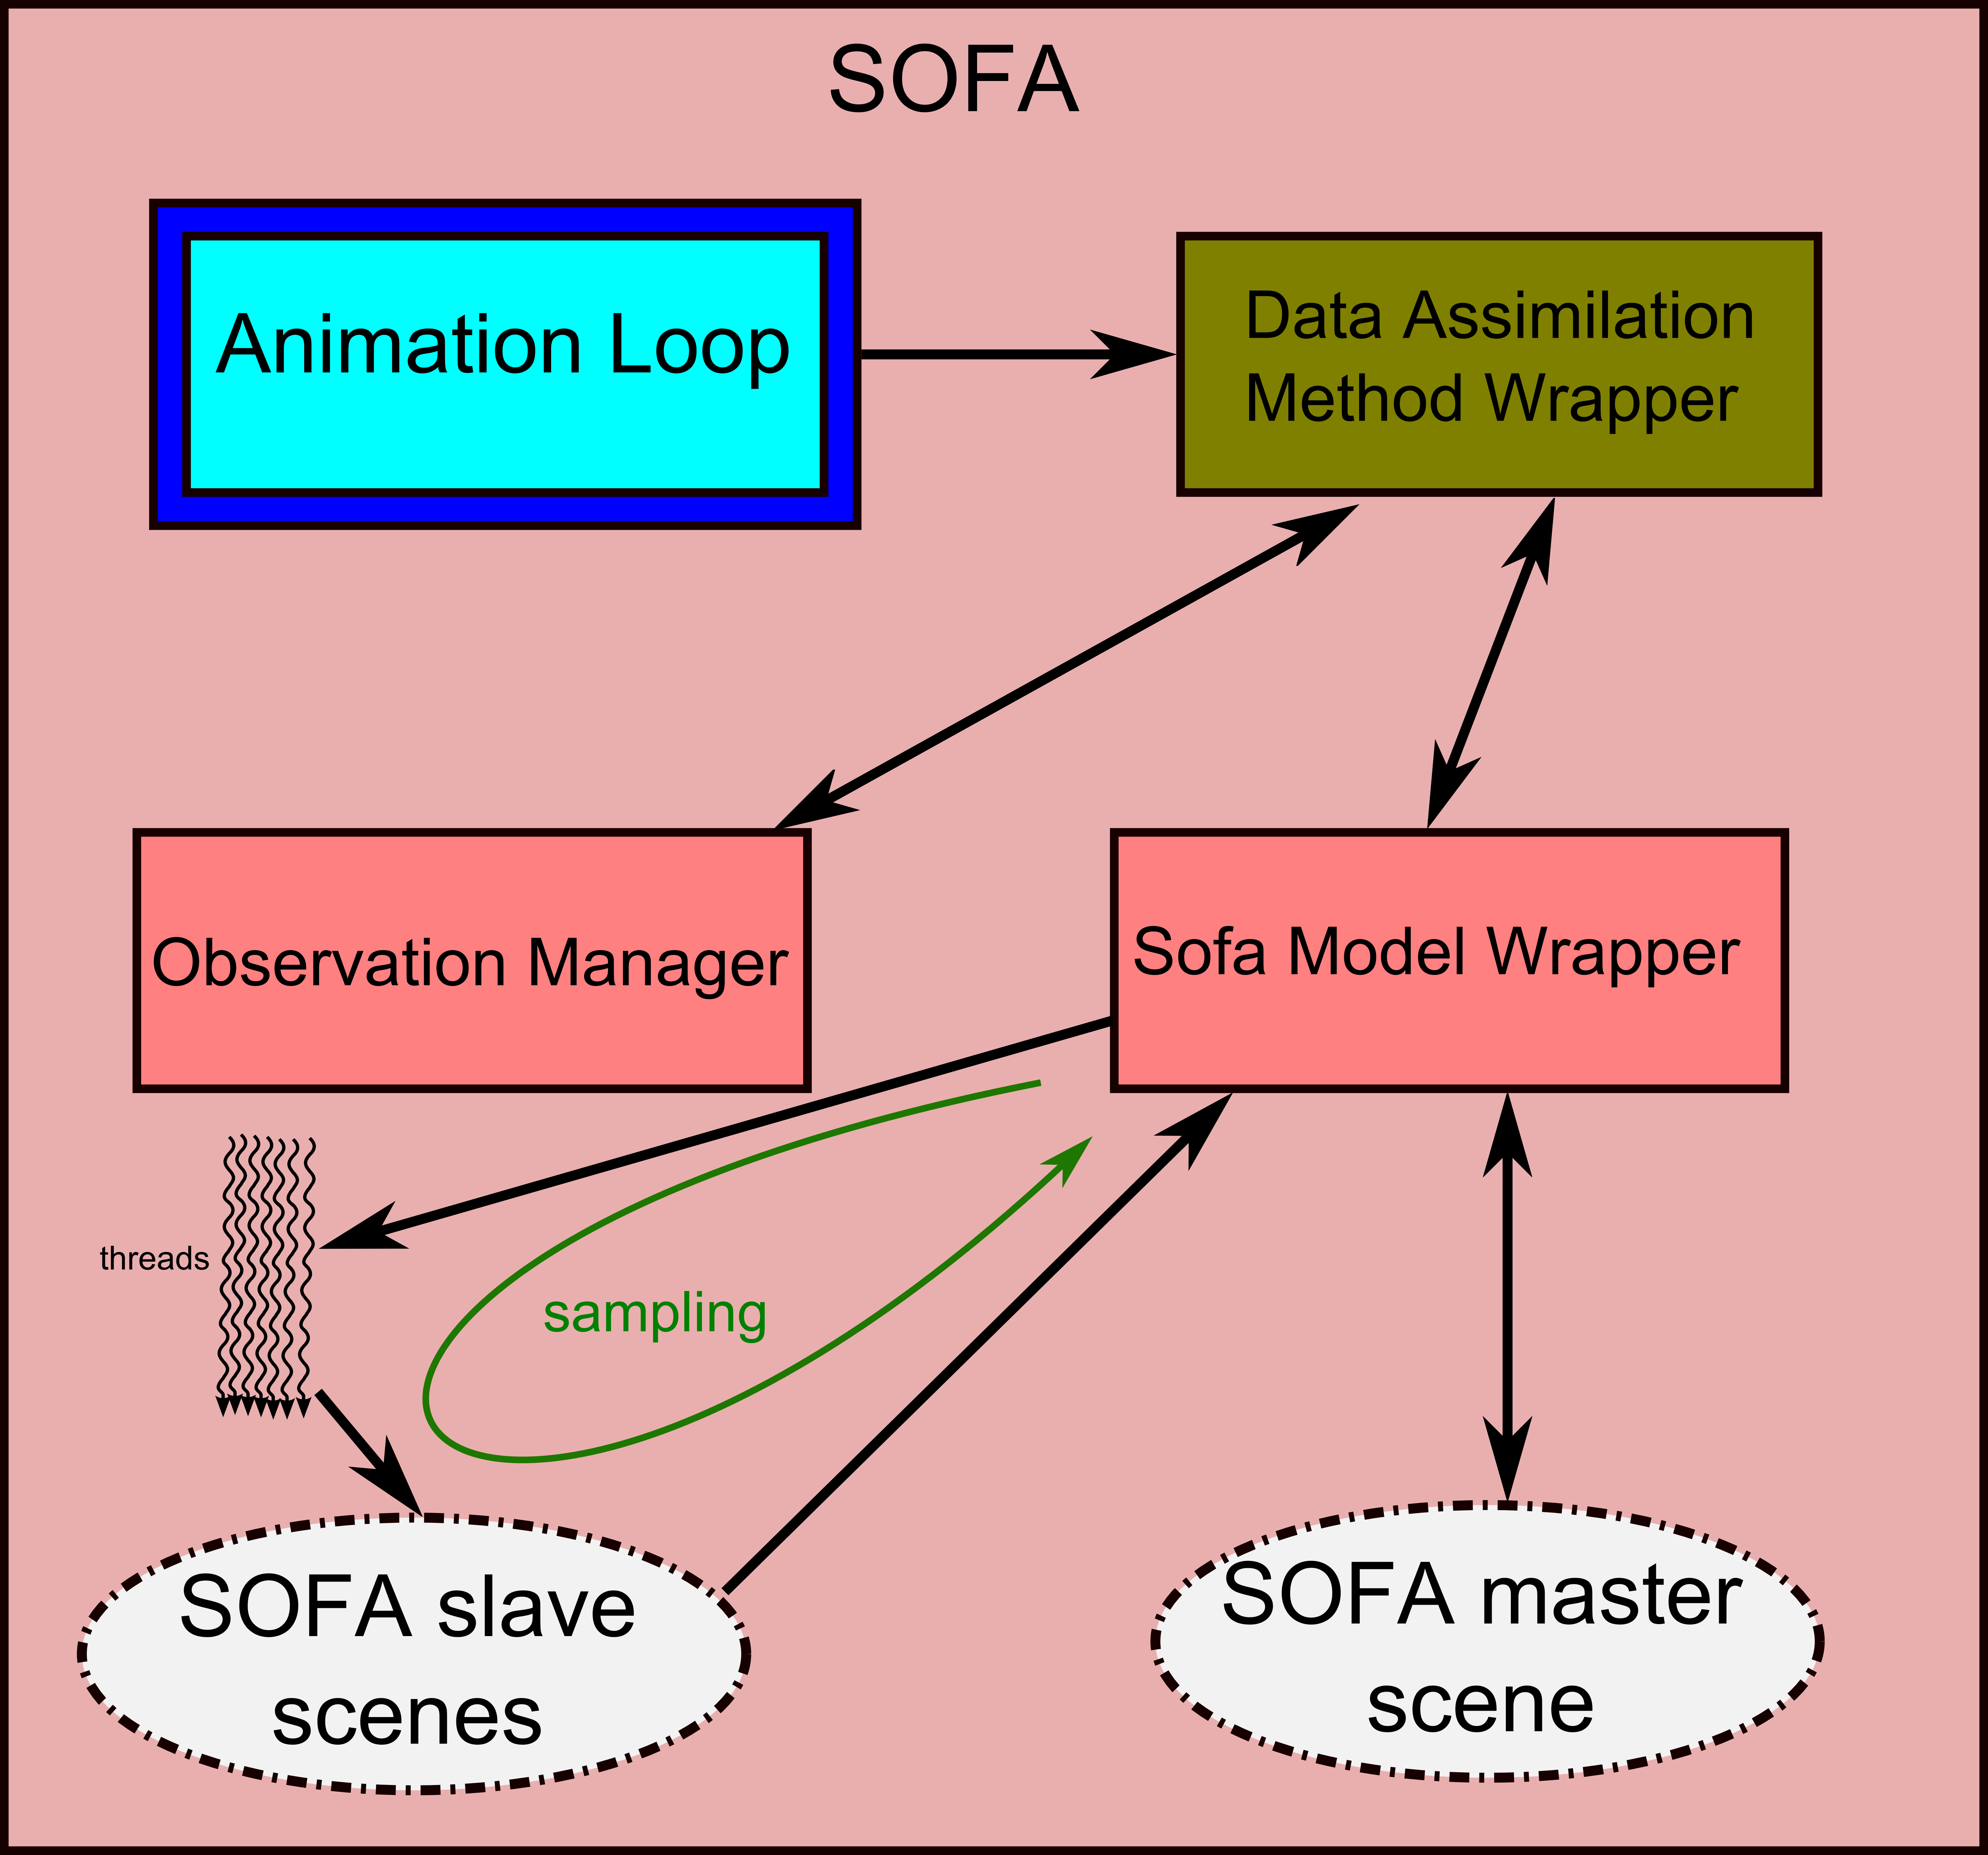
\includegraphics[height=4cm]{figs/integrationScheme2.png}}
\hfill
\subfigure[]{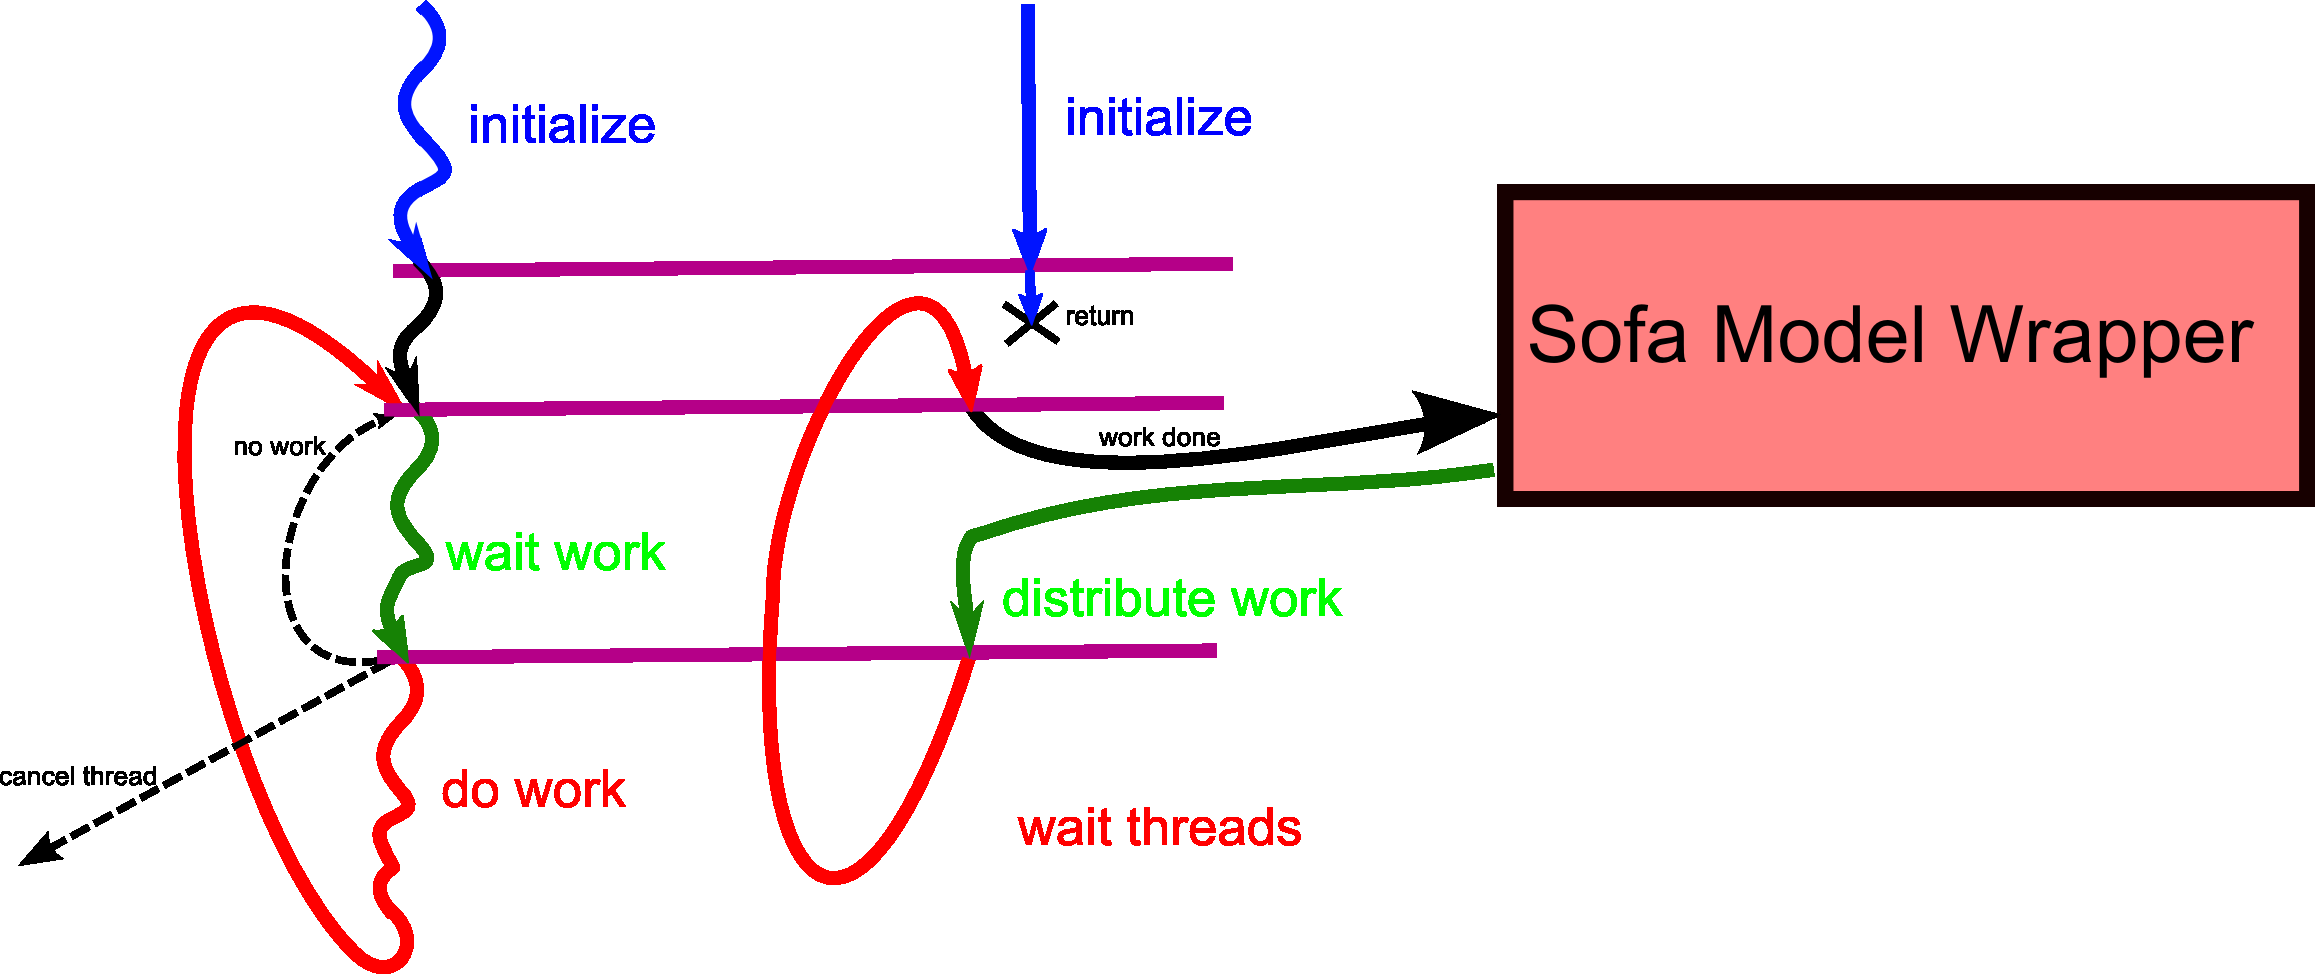
\includegraphics[width=.40\textwidth]{figs/parallelization.png}}
\caption{The schemes depict the integration of SOFA and Verdandi frameworks: (a) The sequential case where the ROUKF invokes the 
model function for each sigma point in a serial manner. (b) The parallel implementation where several instances of the model 
exist and can be evaluated concurrently for different parametrizations. (c) Scheme of the master-slave implementation of the parallel model 
wrapper, where the master thread distribute the work among slaves which execute the actual simulation step for given parametrization.}%
\label{f:integration}
\end{figure*}

\subsection{Reduced-Order Unscented Kalman Filter}
\label{sm:ROUKF}

One of the possible optimizations for large-dimensional systems is based on the observation that the matrix $\mathbf{P}$ is often of reduced rank $d \ll p$. We can then factorize the matrix $\mathbf{P}$ as
\begin{equation*}
\mathbf{P} = \mathbf{L} \mathbf{U}^{-1}\mathbf{L}^{\sf T} \,,
\end{equation*}
where $\mathbf{U}$ is a $d \times d$ invertible matrix -- this matrix then represents the uncertainties in the system. By rewriting the Eq.~\ref{sampling} through \ref{UKFup2} in a way that avoids the direct computation of $\mathbf{P}$, the computational demands decrease considerably. The main benefit is avoiding direct computation of $\mathbf{P}^{-1}$ which, unlike other matrix operations, does not benefit from the sparsity of the matrices. This modification is called \emph{Reduced-order Unscented Kalman Filter} (ROUKF); a detailed description of ROUKF can be found in~\cite{moireau2011reduced}.

%Another room for improvement is the computation of the model step.
%\footnote{Arguably also the measurement step if it were sufficiently computationally intensive.}.
%In an ordinary forward simulation, the simulation steps are inherently sequential and the only room for parallelization is within the individual steps. On the %contrary, the UKF computes $r$ model steps at each simulation step. Considering that the state vector represents the degrees of freedom of the system, the UKF increases the computational complexity by a linear factor. 
%\footnote{For the considered sigma point heuristics featuring O(p) sigma points.}. 
%Furthermore, the computations on different model steps require no coordination --- the task is \emph{embarrassingly parallel} --- and the model step tends to be a rather expensive operation. These facts provide a strong reason to believe that parallelizing the model step computation could provide us with a highly scalable and substantial performance improvement.

\def\bp{\mathbf{p}}
\def\be{\mathbf{e}}
\def\bff{\mathbf{p}}
\def\bfo{\mathbf{p}}
\def\bu{\mathbf{u}}
\def\bx{\mathbf{x}}
\def\bK{\mathbf{A}}
\def\bt{\mathbf{t}}
\def\bR{\mathbf{R}}
\def\bO{\mathbf{O}}
\def\bB{\mathbf{B}}
\def\bL{\mathbf{L}}
\def\bJ{\mathbf{J}}
\def\bF{\mathbf{F}}
\def\br{\mathbf{r}}

\subsection{Model of Deformations}
\label{sm:model}
In this section we provide details about the model which is used in the prediction phase of the ROUKF filter, \ie\ the 
\emph{model function} $f(\mathbf{x})$ called repeatedly in Eq. 5.
In this paper, we consider a physically-based model of deformations which is usually employed for soft-tissue modeling 
in the context of medical simulations.
As we do not focus on the transient part of the deformation, we suppose a quasi-static simulation where 
the actual deformation is given by application of external forces. On the other hand, we aim at modeling large deformations correctly, since
during the surgical interventions, important displacements of tissue occur due to the action of surgical tools.

For this reason we have opted for a finite element method based on a co-rotational formulation introduced by Felippa in~\cite{Felippa2005}, which allows for
large displacements while relying on a linear expression of the stress-strain relationship.
%which respects the rotational invariance needed for correct rendering of large deformations.
The co-rotational approach is based on decomposition of the actual element configuration into rigid rotation and pure deformation, 
both being quantified \wrt~the initial position. More precisely, the actual position of the element nodes
determines the base of the element (given by three chosen adjacent edges), which is both rotated and deformed \wrt\ the initial base of the same element.
In order to extract the rotational component (denoted as $\bR_e$), a matrix decomposition such as polar, SVD or QR is needed;
in our method we employ the technique described in~\cite{Nesme2005}.
The matrix $\bR_\be$ is used to update the local stiffness matrix $\bK_\be$ of the element.
Therefore, via this element-wise rotations, the actual global stiffness matrix $\bK$ depends in each step on the actual deformation $\bu$
and the equation relating the external forces to the displacements can be written as
\begin{equation}
\bK(\bu) = \bfo
%\; \text{ with }  \; \bu = \bx - \bx^0
\label{eq:corotational}
\end{equation}
\noindent where $\bu$ is the vector of displacements and $\bfo$ gathers the applied external forces.
The system represented by Eq.~\ref{eq:corotational} cannot be 
resolved directly due to the non-linearity of $\bK$ \wrt\ $\bu$. Therefore, Newton-Raphson method is employed: 
the system is iteratively solved while in each iteration, linearized \emph{tangent stiffness matrix} $\frac{\partial\bK}{\partial\bu}$ must
be assembled and inverted.

In order to assemble the system matrix $\bK$ and its derivatives, it is necessary to determine mechanical parameters: in the corotational approach considered 
in this paper, the system is parametrized with Poisson's ratio $\nu\in\langle 0,0.5)$ which is the measure of the material compressibility, 
and Young's modulus $E$ [Pa] which quantifies the stiffness of the material. In the context of medical simulations, the Poisson's ratio
close to 0.5 is usually employed. On the other hand, the Young's modulus is a typical representative of a parameter which is patient specific
(as shown for example in~\cite{yeh2002elastic}), nevertheless, it impacts the accuracy of the model significantly.

As we deal with a quasi-static solution, we suppose that 
a sequence of applied external forces $\bfo^{(1)}, \bfo^{(2)}, \ldots, \bfo^{(s)}$ results in a sequence of state vectors
$\bx^{(1)}, \bx^{(2)}, \ldots, \bx^{(s)}$ where $\bx^{(k)} = \bx_0 + \bu^{(k)}$, $\bx_0$ being the vector corresponding to the undeformed initial 
configuration and $\bu^{(k)}$ the displacement computed in $k$-th step of the simulation using Eq.~\ref{eq:corotational}. 

In order to return to the data assimilation scenario, Eq.~\ref{eq:corotational} can be regarded as the model function which transforms 
the actual state of the system represented by the vector of positions $\bx^{(k)}$ into a new state $\bx^{(k+1)}$ as the applied forces
change from $\bfo^{(k)}$ to $\bfo^{(k+1)}$. Since the evaluation of the applied forces is usually smooth, 
the resolution of the non-linear system given by Eq.~\ref{eq:corotational} in step $(k+1)$ can be significantly 
improved by employing the state $\bx^{(k)}$ as the starting configuration of the Newton-Raphson iterative process. 

\begin{figure*}[th]%
\centering%
\subfigure[]{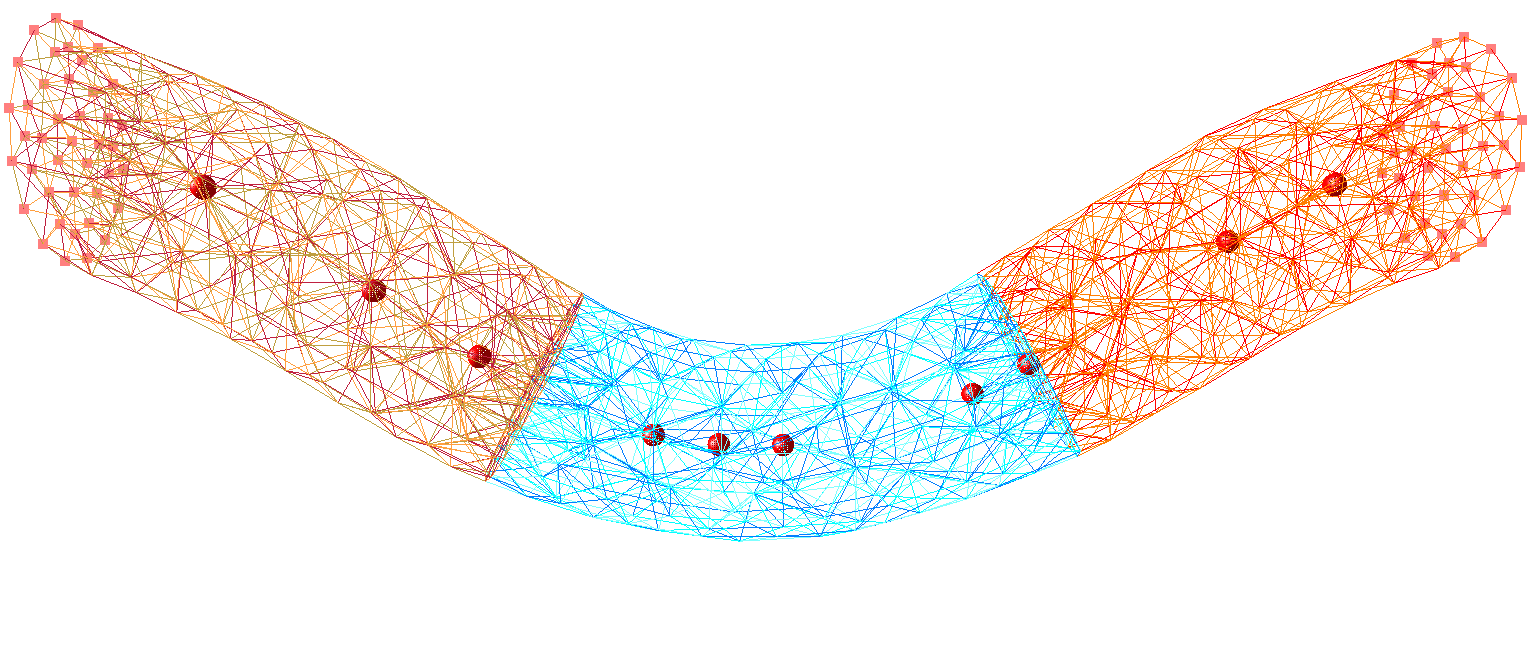
\includegraphics[width=.48\textwidth]{figs/cyl3screen.png}}
\hfill
\subfigure[]{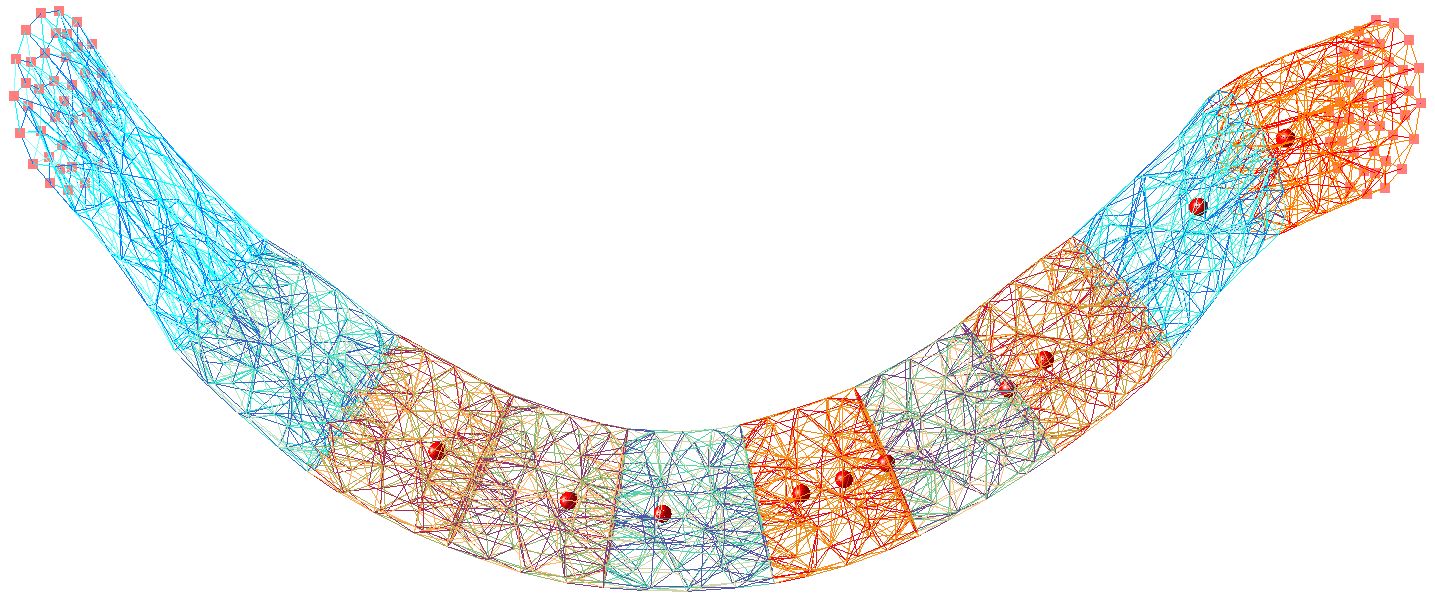
\includegraphics[width=.48\textwidth]{figs/cyl10screen.png}}
\caption{The cylinders used for the evaluation: (a) The mesh $\msa$ composed of 770 elements and 3 segments, with Young's moduli $\{8,2,10\}$\,kPa.
(b) The mesh $\msb$ composed of 4245 elements and 10 segments with Young's moduli $\{1,3,7,6,4,9,5,8,2,10\}$\,kPa}%
\label{f:cylScreens}
\end{figure*}

\section{Implementation}
\label{s:implement}

\subsection{Frameworks}
\label{si:frameworks}
In order to integrate the concepts of data assimilation based on reduced-order Kalman filtering, and the physics-based 
simulation of elastic deformations, we performed an integration of two frameworks. 

Simulation Open Framework Architecture (SOFA)~\footnote{\url{http://www.sofa-framework.org/}} is an open-source framework, written in C++. 
It primarily targets on the real-time simulation of deformable bodies and fluids, with an emphasis on medical simulation.
The framework allows for complicated simulation scenarios, benefiting from the possibility of creating complex 
scenes composed of hierarchically organized nodes populated by components. Each component represents a single functionality; for further details 
we refer the reader to~\cite{faure2012sofa}. It should be noted that a simulation in SOFA is always driven by an \emph{animation loop} 
which recursively calls visitors responsible for correct employment of different components. 

Verdandi~\footnote{\url{http://verdandi.sourceforge.net/}} is a generic, open-source library, written in C++. 
It aims at providing various methods and tools for data assimilation (DA) and currently consists of eight data assimilation methods
including EKF, UKF, ROEKF (a reduced-order variant of the EKF) and finally ROUKF. 
Verdandi is designed to be useful for a large variety of high-dimensional numerical models~\cite{chabiniok2012}. 

\subsection{Integration}
\label{si:integration}
Unlike a standard simulation where a new state is computed from the previous one by a single application of a model function (such as the one described in 
section~\ref{sm:model}), the data assimilation process based on the ROUKF presented in~\ref{sm:ROUKF} requires multiple evaluations 
of the model function, \ie\ it calls the model function with different parametrizations each corresponding to 
one sigma point. In order to perform the integration of SOFA (representing the model) and Verdandi (representing the driving filter), 
we have implemented a new animation loop which hands-over the control to the ROUKF. 
The filter executes the process described by Eq.~4 to 13 and it holds that
\begin{itemize}
\item In the prediction phase, it invokes a SOFA component called \emph{model wrapper} which is an abstraction of the SOFA functionality implementing the model function $f$ (Eq. 5) executed for each sigma point.
\item In the correction phase, it calls an \emph{observation manager} which implements the computation of innovation function $h$ (Eq. 8).
\end{itemize}
The scheme of the implementation is depicted in Fig.~\ref{f:integration}(a). 

\subsection{Parallel Sampling}
\label{si:parallel}
The algorithmic design of the ROUKF offers a great opportunity for parallelization of the sampling phase (evaluation of the model function 
for sigma points), as the task is embarrassingly parallel.
The parallelisation was implemented using Pthreads library which
appears to suit well the purpose and provides a performance at least similar to that of other options. 

The main issue related to the parellelization is given by the fact that unlike the sequential version where a single instance of the 
assimilated object is sufficient, the parallel version requires an independent instance for each thread. In reality, this 
means that at the beginning of the assimilation process, the simulation scene must be replicated so that $t-$ slave instances 
of the same object can be called independently by corresponding threads in order to evaluate the model function for given sigma point. 
The concept is presented in Fig.~\ref{f:integration}(b) where the model wrapper represent the same abstraction as before, however, it allows
 for multiple concurrent evaluation of the underlying simulation scene. 
 
 Since it cannot be assumed that the number of threads is equal to the number of sigma points, the evaluation of the model function 
 is assigned to the threads by a master thread. Since the workload performed by the slave threads can vary according to the number of
 processed sigma points and the length of computation of single model function, the threads are synchronized using a barrier at the end 
 of parallel sampling. The implementation is schematically depicted in Fig.~\ref{f:integration}(c). 








